% s1_aft cut, because I apparently need to include this

\chapter{Data selection using s1\_area\_fraction\_top}\label{app:s1aft}

\section{Introduction}

For each peak recorded in the XENON1T detector, a wide variety of properties are computed. One of these is the \textit{area\_fraction\_top}, which is the fraction of the peak's area measured by the top PMT array. While this quantity is largely constant for all S2 peaks (due to the tightly-constrained space in \textit{z} where the S2s are generated), for S1 peaks this quantity can change significantly. This can be used as a verification for the reconstructed \textit{z} coordinate of the interaction by comparing the measured \textit{s1\_area\_fraction\_top} to the expected value, given the reconstructed location vertex.

\section{area\_fraction\_top throughout the detector}

First we must determine, at all points in the detector, what the probability is that a photon created will be observed by the top array. While this is entirely geometrically determined, other factors such as reflection from the walls and total internal reflection off the liquid surface mean it is easier to determine this relationship from data. Monoenergetic lines are ideal for this, but they should be at sufficiently low energy so PMT saturation is not a significant concern. The $32\1{keV}$ line from $^{83m}$Kr is ideal for this, as only about 250 photons are detected from this peak.

\subsection{Event selection}

Events are selected from the XENON1T SR1 $^{83m}$Kr calibration data. Two S1s are required, the first between 210 and 300 PE, the second between 63 and 113 PE, as shown in Figure~\ref{fig:s1a_s1b}. Furthermore, the reconstructed positions of the two interactions involving these two S1s are required to be within $1\1{mm}$ of each other.

\begin{figure}[htb]
    \centering
    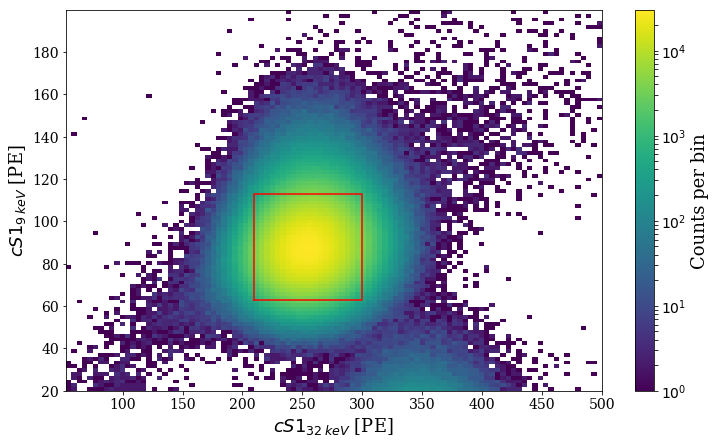
\includegraphics[width=0.8\textwidth]{figures/app_s1aft/sr1_83mkr_s1s}
    \caption{The double-decay structure of $^{83m}$Kr makes selection of events with resolved S1s very straightforward. 